\chapter{Nuclear Physics}
In this chapter, all units are SI with the exception of: temperature
and energy, which are defined in the historical units of eV
(electron-volts); cross sections, which are defined in the historical
units of barn; and Bosch-Hale reaction rates, which are given in cubic
centimeters per second.\\

\noindent
$e$ is the elementary electric charge\\
$Z$ is the number of nuclear protons\\
$N$ is the number of nuclear neutrons\\
$A$ is the number of nucleons (N+Z)\\
$m$ is the particle mass\\
$n$ is the particle number density\\
$\mathbf{v}$ is the particle velocity vector\\
$E$ is the particle kinetic energy\\


% Reference for reaction and Q Values - Brookhaven NNDC ENDF-VII.3 (2009)
\section{Fundamental Definitions}
Nuclear reaction notation \scite{krane}{378-381}
\fla{ 
  \begin{gathered}
    a+X\Rightarrow b+Y \\
    \text{or} \\
    X(a,b)Y \\
  \end{gathered}
  \hspace{0.3cm} \text{where} \hspace{0.3cm}
  \left\{
  \begin{gathered}
    a = \text{bombarding particle} \hfill\\      
    X = \text{target nucleus} \hfill\\
    b = \text{ejected particle(s)} \hfill\\
    Y = \text{product nucleus} \hfill\\
  \end{gathered}
  \right.
  &
  \begin{gathered}
    \left\} 
    \begin{gathered}
      \text{entrance channel}\\
      \\
    \end{gathered}
    \right.
    \\
    \left\} 
    \begin{gathered}
      \text{exit channel} \\
      \\
    \end{gathered}
    \right.
  \end{gathered}
}

\begin{table}[H]
  \begin{tabular}{l l}
    X(a,b)Y & general nuclear reaction\\
    X(a,a)X & elastic scattering\\
    X(a,a')X* & inelastic scattering\\
    X(n,n)X & neutron elastic scattering\\
    X(n,n')X* & neutron inelastic scattering\\
    X(n,2n)Y & neutron multiplication\\
    X(n,$\gamma$)Y & neutron capture\\
    X(n,f)Y & neutron-induced fission\\
  \end{tabular}
  \end{table}

\index{Semi-empirical mass formula}
\index{Nuclear mass}
\noindent
Nuclear mass \scite{krane}{65}
\fla{ m &= Zm_p + Nm_n - E_B/c^2 &}

\index{Nuclear binding energy}
\noindent
Nuclear binding energy  \scite{krane}{68}
\fla{ E_B(A,Z) &= a_vA - a_s A^{2/3} - a_c\frac{Z(Z-1)}{A^{1/3}} - a_a\frac{(A-2Z)^2}{A} + \delta(A,Z) &}
\indent
where the value of the coefficients $a$ in MeV is \scite{krane}{68}
\fla{a_v &= 15.5 & a_s &= 16.8 & a_c &= 0.72 & a_a &= 23 & a_p&= 34\text{ MeV}  &}
\fla{
  \delta(A,Z) &= \left\{
  \begin{gathered}
    a_p A^{-3/4}  \hfill \text{(Z,N even)}\\
    0 \hfill \text{(A odd)}\\
    -a_p A^{-3/4} \hspace{0.5cm} \text{(Z,N odd)}\\
  \end{gathered} \right.
  &\\
}

\index{Q! Nuclear reactions}
\noindent
Nuclear reaction Q-value \scite{krane}{381}
\fla{ Q &= \left( (m_a+m_X) - (m_b+m_Y)\right)c^2 = E_f - E_i &}

\index{Reaction threshold energy}
\noindent
Reaction threshold energy ($Q<0$) \scite{krane}{382}
\fla{ E_\mathrm{thresh} &= -\left(\frac{m_Y+m_b}{m_y+m_b-m_a}\right)Q \approx -\left(1 + \frac{m_a}{m_X}\right)Q &}

\index{Nuclear Interactions}
\section{Nuclear Interactions}
$A\equiv m_A/{m_N}$ is approximately the nucleus atomic mass number \\
$i$ and $f$ refer to initial and final, respectively\\
$\theta$ is the angle between the $a$ and $b$ trajectory in the lab frame\\
$\theta_\mathrm{cm}$ is the angle between the $a$ and $b$ trajectory in the center of mass frame\\

\noindent
Reaction Q-value from kinematics \scite{krane}{384}
\fla{ Q &= E_b\left(1+\frac{m_b}{m_Y}\right) - E_a\left(1-\frac{m_a}{m_Y}\right) - 2\left(\frac{m_a m_b}{m_Y^2}E_aE_b\right)^{1/2}\cos\theta &}

\noindent
Ejected particle energy: X(a,b)Y \scite{krane}{382}
\fla{ E_y^{1/2} &= \zeta \frac{\left(m_a m_b E_a\right)^{1/2}}{m_Y+m_b} \pm \frac{\left(m_a m_b E_a\zeta^2 + (m_Y+m_b)[m_YQ+(m_Y-m_a)E_a]\right)^{1/2}}{m_Y+m_b} &}

\noindent
Maximum kinetic energy transfer fraction: X(a,a)X~~\cite{authors}
\fla{ \left. \frac{E_f}{E_i}\right|_{\theta=0} &= \frac{4A_1A_2}{\left(A_1+A_2\right)^2} &}

\index{Charged particle interactions}
\subsection{Charged Particle Interactions}

\index{Stopping power}
\index{Bethe formula}
Stopping power of heavy charged particles (Bethe formula) \scite{krane}{194}
\fla{ \frac{dE}{dx} &= \left(\frac{e^2}{4\pi\epsilon_0}\right)^2\frac{4\pi z^2N_AZ\rho}{m_ec^2\beta^2A}\left[\ln\left(\frac{2m_ec^2\beta^2}{I}\right)-\ln\left(1-\beta^2\right)-\beta^2\right] &}
\indent where $\beta c=v$ and $ze$ are the incident particle's speed and charge; \\
\indent $\rho$ is the mass density of the stopping medium;\\
\indent $N_A$ is Avogadro's number;\\
\indent $I$ is mean excitation of atomic electrons, typically taken as $I\approx10Z$.\\

\noindent
Collisional stopping power of electrons \scite{krane}{196}
\fla{ \left(\frac{dE}{dx}\right)_c &= \left(\frac{e^2}{4\pi\epsilon_0}\right)^2\frac{2\pi N_A Z \rho}{m_ec^2\beta^2A}\left[\ln\frac{E_i(E_i+m_ec^2)^2\beta^2}{2I^2m_ec^2}+\left(1-\beta^2\right)\right. & \\
                             & \left. - \left(2\sqrt{1-\beta^2}-1+\beta^2\right)\ln 2 + \frac{1}{8}\left(1-\sqrt{1-\beta^2}\right)^2 \right] &}

\noindent
Radiative stopping power of electrons ($\gtrsim1~\mathrm{MeV}$) \scite{krane}{196}
\fla{ \left(\frac{dE}{dx}\right)_r &= \left(\frac{e^2}{4\pi\epsilon_0}\right)^2\frac{Z^2N_A\left(E_i+m_ec^2\right)\rho}{137m_e^2c^4A}\left[4\ln\frac{2\left(E_i+m_ec^2\right)}{m_ec^2}-\frac{4}{3}\right] &}

\index{Neutron interactions}
\subsection{Neutron Interactions}

% \index{Neutron scattering}
% \noindent
% I believe that this comes from the ``Ion Beam Bible'' by Tesmer et al (ZSH 19 OCT 11)
% Ejected neutron energy: X(n,b)Y %\scite{Tesmer}
% \fla{ E_{n,f}^{1/2} &= (1+A)^{-2}\left\{E_{n,i}^{1/2}\zeta \pm \left[E_{n,i}\left(A^2-1+\zeta\right)+A\left(A+1\right)Q\right]^{1/2}\right\}^{1/2} &}

\noindent
Ejected neutron energy: X(n,n)X \scite{krane}{448}
\fla{ E_{n,f} &= \frac{A^2+2A\cos\theta_\mathrm{cm}+1}{\left(A+1\right)^2} &}

\noindent
Maximum kinetic energy transfer fraction: X(n,n)X \scite{krane}{448}
\fla{ \left.\frac{E_{n,f}}{E_{n,i}}\right|_{\theta=0} &= \left(\frac{A-1}{A+1}\right)^2 \hspace{0.5cm}&}

\index{Neutron lethargy}
\noindent
Neutron lethargy (E$_n \lesssim$ 10 MeV) \scite{krane}{450}
\fla{ \xi &=1+\frac{(A-1)^2}{2A}\ln\left(\frac{A-1}{A+1}\right) &}

\noindent
Number of collisions required to change neutron energies \scite{krane}{450}
\fla{ N &= \frac{\ln(E_i/E_f)}{\xi} &}

\index{Gamma interactions}
\subsection{Gamma Interactions}

\index{Klein-Nishina cross section}
\noindent
Klein-Nishina cross section for Compton scattering \scite{krane}{201}
\fla{ \frac{d\sigma}{d\Omega} &= r_0^2 \left[\frac{1}{1+\alpha\left(1-\cos\theta\right)}\right]^3 \left[\frac{1+\cos^2\theta}{2}\right]\left[1+\frac{\alpha^2\left(1-\cos\theta\right)}{\left(1+\cos^2\theta\right)\left[1+\alpha\left(1-\cos\theta\right)\right]}\right] &}
\indent where $(\alpha=E_\gamma/mc^2)$ and $(r_0=e^2/4\pi\epsilon_0mc^2=2.818~\mathrm{fm})$ is the classical \\ \indent electron radius.\\

\index{Compton scattering}
\index{Classical electron radius}
\noindent
Energy shift from Compton scattering \scite{krane}{201}
\fla{ E_f &= \frac{E_i}{1+\left(\frac{E_i}{mc^2}\right)\left(1-\cos\theta\right)} &}


\section{Cross Section Theory}
A reaction cross section $\sigma(E_a)$, or more simply $\sigma$, is a
measure of the probability that reaction $X(a,b)Y$ will occur.
Consider a beam of $a$ particle with current $I_a$ directed onto $X$
target nuclei with an areal density of $N_X$ per unit area.  By
observing the energy and angular distribution, $e(E_b)$ and
$r(\theta,\phi)$ respectively, of the ejected particle $b$ into a
solid angle $d\Omega$ then the doubly differential cross section can
be determined, which is the probability of observing particle $b$ at
in solid angle $d\Omega$ with energy $E_b$. \scite{krane}{392-394}
\newline
\newline

\index{Cross sections! Definitions}
\noindent
Doubly differential cross section \scite{krane}{392-393}
\fla{ \frac{d\sigma}{d\Omega\,dE_b} =& \frac{r(\theta,\phi)~e(E_b)}{4\pi I_aN_X} &}

\noindent
Differential energy cross section \scite{krane}{393}
\fla{ \frac{d\sigma}{dE_b} &= \int \frac{d\sigma}{d\Omega\,dE_b} d\Omega &}

\noindent
Differential angular cross section \scite{krane}{393}
\fla{ \frac{d\sigma}{d\Omega} &= \int \frac{d\sigma}{d\Omega\,dE_b}\,dE_b &}

\noindent
Reaction cross section \scite{krane}{393}
\fla{ \sigma &= \int \frac{d\sigma}{d\Omega}\, d\Omega 
  = \int \limits_0^{2\pi} \!\! \int \limits_0^{\pi} \frac{d\sigma}{d\Omega} \,\sin\theta\,d\theta\,d\phi &}

\noindent
Total cross section \scite{krane}{393}
\fla{ \sigma_{T} &=\!\!\!\!\!\!\! \sum \limits_{i=0}^{\text{all reactions}} \!\!\!\!\!\!\! \sigma_i &}

\index{Sommerfeld parameter}
\noindent
The Sommerfeld parameter \scite{thompson}{5}
\fla { \eta &= \frac{Z_aZ_Xe^2}{\hbar v} &}

\index{Astrophysical S-factor}
\noindent
Astrophysical S-factor \scite{thompson}{5}
\fla{ S(E) &= \sigma(E)E \exp\left(2\pi\eta\right) &}


\index{Reaction rates! Definitions in plasma}
\section{Reaction Rate Theory}
For a thermonuclear plasma, the volumetric reaction rate $\mathcal{R}$
(also known as \textit{thermal reactivity}) describes the number of
reactions occuring per unit volume per unit time.  In thermonuclear
fusion plasmas, $\mathcal{R}$ is obtained by integrating the
energy-dependent cross section, $\sigma(v)$, over the distribution
functions of the participating species. \scite{wesson}{5-8}
\newline
\newline
\noindent
Partial volumetric reaction rate \scite{wesson}{5-6}
\fla{
  \mathcal{R}_p &= \sigma(v)vf_1(\textbf{v}_1)f_2(\textbf{v}_2)
  \hspace{0.5cm}\textbf{v} = \textbf{v}_1 - \textbf{v}_2 &
}

\noindent
Total volumetric reaction rate for general $f(v)$ \scite{wesson}{6}
\fla{ \mathcal{R} &= \frac{1}{1+\delta_{12}}\iint
  \sigma(v)vf_1(\textbf{v}_1)f_2(\textbf{v}_2) \,d^3v_1\,d^3v_2 &}
\indent where $\delta_{12}$ is the Kronecker delta for particle species 1 and 2 that prevents \\
\indent double counting for like-species plasmas.\\

\noindent
Total volumetric reaction rate for Maxwellian $f(v)$) \scite{bosch}{624} \scite{wesson}{6} 
\fla{
  \mathcal{R} &= \frac{n_1n_2}{1+\delta_{12}}\langle\sigma v\rangle
  \text{  where  }
  \left\{
  \begin{gathered}
    \langle\sigma v\rangle = \left(\frac{8\mu^3}{\pi T^3}\right)^{1/2}\frac{1}{m_1^2} \int \sigma(E)Ee^{-\mu E/m_1T}\,dE \text{   \tiny[m$^3$s$^{-1}$}] \hfill\\
    \hfill \mu = \frac{m_1m_2}{m_1 + m_2} \hspace{2cm} E = \frac{1}{2}mv^2 \hfill\\
  \end{gathered}
  \right.
  &
}


\vfill

\pagebreak
\section{Nuclear Reactions for Fusion Plasmas}
\noindent
All data from the ENDF/B-VII nuclear data libraries.\cite{chadwick}
\begin{table}[h!]\small
  \centering
  \begin{tabular}{l r c l c c}
    \multicolumn{6}{c}{Abbreviations: n=neutron, p$=^1$H, d$=^2$H, t$=^3$H, h=$^3$He, $\alpha=^4$He}\\
    \hline
    & Reactants \T & & Products & Branching & Q-value \\[5pt]
    &           \B & & (kinetic energy in MeV) & ratio & (MeV) \\[5pt]
    \hline\hline
    1.\T & d + t        & $\longrightarrow$ & $\alpha$(3.52) + n(14.07) & 1.00  & 17.59 \\[5pt]
    2.   & d + d        & $\longrightarrow$ & t(1.01) + p(3.02)         & 0.50  &  4.03 \\[5pt]
         &              & $\longrightarrow$ & h(0.82) + n(2.45)         & 0.50  &  3.27 \\[5pt]
    3.   & d + h        & $\longrightarrow$ & $\alpha$(3.67) + p(14.68) & 1.00  & 18.35 \\[5pt]
    4.   & t + t        & $\longrightarrow$ & $\alpha$ + 2n             & 1.00  & 11.33 \\[5pt]
    5.   & h + t        & $\longrightarrow$ & $\alpha$ + p + n          & 0.51  & 12.10 \\[5pt]
         &              & $\longrightarrow$ & $\alpha$(4.77) + d(9.54)  & 0.43  & 14.32 \\[5pt]
         &              & $\longrightarrow$ & $^5$He(1.87) + p(9.34)    & 0.06  & 11.21 \\[5pt]
    6.   & p + $^6$Li   & $\longrightarrow$ & $\alpha$(1.72) + h(2.30)  & 1.00  &  4.02 \\[5pt]
    7.   & p + $^7$Li   & $\longrightarrow$ & 2 $\alpha$                & 0.20  & 17.35 \\[5pt]
         &              & $\longrightarrow$ & $^7$Be + n                & 0.80  & -1.64 \\[5pt]
    8.   & d + $^6$Li   & $\longrightarrow$ & 2 $\alpha$                & 1.00  & 22.37 \\[5pt]
    9.\B & p + $^{11}$B & $\longrightarrow$ & 3 $\alpha$                & 1.00  &  8.62 \\[5pt]
    \hline
  \end{tabular}
  \label{plasmaReactions}
\end{table}

\section{Nuclear Reactions for Fusion Energy}
\noindent
All data from the ENDF/B-VII nuclear data libraries.\cite{chadwick}
\begin{table}[h!]\small
  \centering
  \begin{tabular}{l c c c c c}
    \multicolumn{6}{c}{Abbreviations: n=neutron, t=$^3$H, B=tritium breeding, M=neutron multiplication}\\
    \hline
    & Reaction \T\B & Q-value & Purpose & $\sigma(0.025\mathrm{~eV})$ & $\sigma(14.1\mathrm{~MeV})$ \\[5pt]
    &               & [MeV]   &         & [barn]                          & [barn] \\[5pt]
    \hline\hline
    1. \T& $^6$Li(n,t)$^4$He           &  4.78  & B   & 978   & 0.03\\[5pt]
    2.   & $^6$Li(n,2n$\alpha$)$^6$Li  & -3.96  & M   & -     & 0.08\\[5pt]
    3.   & $^7$Li(n,2n)$^6$Li          & -7.25  & M   & -     & 0.03\\[5pt]
    4.   & $^7$Li(n,2n$\alpha$)$^3$H   & -8.72  & B/M & -     & 0.02\\[5pt]
    5.   & $^9$Be(n,2n)$^8$Be          & -1.57  & M   & -     & 0.48\\[5pt]
    6.   & $^{204}$Pb(n,2n)$^{203}$Pb  & -8.39  & M   & -     & 2.22\\[5pt]
    7.   & $^{206}$Pb(n,2n)$^{205}$Pb  & -8.09  & M   & -     & 2.22\\[5pt]
    8.   & $^{207}$Pb(n,2n)$^{206}$Pb  & -6.74  & M   & -     & 2.29\\[5pt]
    9. \B& $^{208}$Pb(n,2n)$^{207}$Pb  & -7.37  & M   & -     & 2.30\\[5pt]
    \hline
  \end{tabular}
  \label{breederReactions}
\end{table}

\vfill

\pagebreak
\index{Cross sections! Parametrization}
\section{Fusion Cross Section Parametrization}
The Bosch-Hale parametrization of the fusion reaction cross section~~\cite{bosch}
\fla{ \sigma(E_\mathrm{keV}) &= \frac{S(E)}{E\exp(B_G/\sqrt{E})} \hspace{0.5cm} \mathrm{[millibarn]} &}
\indent
where
\fla{ S(E_\mathrm{keV}) &= \frac{A_1+E(A_2+E(A_3+E(A_4+EA_5)))}{1+E(B_1+E(B_2+E(B_3+EB_4)))} &}

% REFERENCE: Bosch and Hale, Nucl. Fus. 32 (1992) 611
\noindent
\begin{table}[h!]\small
  \noindent
  \centering
  \begin{tabular}{c c c c c}
    \multicolumn{5}{c}{Bosch-Hale parametrization coefficients for several fusion reactions~\cite{bosch}}\\
    \hline
    \T\B& $^2$H(d,n)$^3$He & $^2$H(d,p)$^3$H & $^3H$(d,n)$^4$He & $^3$He(d,p)$^4$He\\
    \hline\hline
    B$_G$ [keV]\T\B& 31.3970 & 31.3970 & 34.3827 & 68.7508 \\
    \hline
            % 2H(d,n)                    % 2H(d,p)                      % 3H(d,n)                    % 3He(d,p)
    A$_1$\T& 5.3701$\times$10$^4$        & 5.5576$\times$10$^4$      & 6.927$\times$10$^4$      & 5.7501$\times$10$^6$ \\ 
    A$_2$    & 3.3027$\times$10$^2$      & 2.1054$\times$10$^2$      & 7.454$\times$10$^8$      & 2.5226$\times$10$^3$ \\
    A$_3$    & -1.2706$\times$10$^{-1}$  & -3.2638$\times$10$^{-2}$  & 2.050$\times$10$^6$      & 4.5566$\times$10$^1$ \\
    A$_4$    & 2.9327$\times$10$^{-5}$   & 1.4987$\times$10$^{-6}$   & 5.200 $\times$10$^4$     & 0.0 \\
    A$_5$  \B& -2.5151$\times$10$^{-9}$  & 1.8181$\times$10$^{-10}$  & 0.0                      & 0.0 \\
    \hline
    B$_1$\T& 0.0                         & 0.0                       & 6.380 $\times$10$^1$     & -3.1995$\times$10$^{-3}$ \\
    B$_2$    & 0.0                       & 0.0                       & -9.950$\times$10$^{-1}$  & -8.5530$\times$10$^{-6}$ \\
    B$_3$    & 0.0                       & 0.0                       & 6.981 $\times$10$^{-5}$  & 5.9014$\times$10$^{-8}$ \\
    B$_4$\B & 0.0                        & 0.0                       & 1.728 $\times$10$^{-4}$  & 0.0\\
    \hline
    Valid Range [keV] \T\B& 0.5$<$E$<$4900 & 0.5$<$E$<$5000 & 0.5$<$E$<$550 & 0.3$<$E$<$900 \\
    \hline
  \end{tabular}
  \label{table:xsParam}
\end{table}

\index{Cross sections! Tabulated values}
\noindent
\begin{table}[h!]\small
  \noindent
  \centering
  \begin{tabular}{c c c c c}
    \multicolumn{5}{c}{Tabulated Bosch-Hale cross sections [millibarns]~~\cite{bosch}}\\
    \hline
    E (keV) \T\B& $^2$H(d,n)$^3$He & $^2$H(d,p)$^3$H & $^3H$(d,n)$^4$He & $^3$He(d,p)$^4$He\\
    \hline\hline
    3\T& 2.445$\times$10$^{-4}$ & 2.513$\times$10$^{-4}$ & 9.808$\times$10$^{-3}$ & 1.119$\times$10$^{-11}$ \\ 
    4 & 2.093$\times$10$^{-3}$ & 2.146$\times$10$^{-3}$ & 1.073$\times$10$^{-1}$ & 1.718$\times$10$^{-9}$ \\ 
    5 & 8.834$\times$10$^{-3}$ & 9.038$\times$10$^{-3}$ & 5.383$\times$10$^{-1}$ & 5.199$\times$10$^{-8}$ \\
    6 & 2.517$\times$10$^{-2}$ & 2.569$\times$10$^{-2}$ & 1.749$\times$10$^0$    & 6.336$\times$10$^{-7}$ \\
    7 & 5.616$\times$10$^{-2}$ & 5.720$\times$10$^{-2}$ & 4.335$\times$10$^0$    & 4.373$\times$10$^{-6}$ \\
    8 & 1.064$\times$10$^{-1}$ & 1.081$\times$10$^{-1}$ & 8.968$\times$10$^0$    & 2.058$\times$10$^{-5}$ \\
    9 & 1.794$\times$10$^{-1}$ & 1.820$\times$10$^{-1}$ & 1.632$\times$10$^1$    & 7.374$\times$10$^{-5}$ \\
   10 & 2.779$\times$10$^{-1}$ & 2.812$\times$10$^{-1}$ & 2.702$\times$10$^1$    & 2.160$\times$10$^{-4}$ \\
   12 & 5.563$\times$10$^{-1}$ & 5.607$\times$10$^{-1}$ & 6.065$\times$10$^2$    & 1.206$\times$10$^{-3}$ \\
   15 & 1.178$\times$10$^{0}$  & 1.180$\times$10$^{0}$  & 1.479$\times$10$^2$    & 7.944$\times$10$^{-3}$ \\
   20\B& 2.691$\times$10$^{0}$  & 2.670$\times$10$^{0}$  & 4.077$\times$10$^2$    & 6.568$\times$10$^{-2}$ \\
   \hline
  \end{tabular}
  \label{table:xs}
\end{table}

\vfill

\pagebreak
\index{Reaction rates! Parametrization}
\section{Fusion Reaction Rate Parametrization}

\noindent
The Bosch-Hale parametrization of the volumetric reaction rates~~\cite{bosch}

\fla{ \langle\sigma v\rangle &= C_1 \cdot \theta \cdot \sqrt{\frac{\xi}{m_\mu c^2T_\mathrm{i,~keV}^3}}\,e^{-3\xi} \hspace{0.5cm}
  \begin{gathered}
    \mathrm{[cm^3~s^{-1}]}\\
    \tiny or \normalsize\\
    \mathrm{\times10^{-6}\,\,\mathrm{[m^3~s^{-1}]}}\\
  \end{gathered}
  &}
\indent
where
\flatwo{ \theta &= T / \left(1-\frac{T(C_2+T(C_4+TC_6))}{1+T(C_3+T(C_5+TC_7))}\right) & \xi &= \left(\frac{B_G^2}{4\theta}\right)^{1/3}}{1}

\begin{table}[h!]\small
  \noindent
  \centering
  \begin{tabular}{c c c c c}
    \multicolumn{5}{c}{Bosch-Hale parametrization coefficients for volumetric reaction rates~~\cite{bosch}}\\
    \hline
    \T\B& $^2$H(d,n)$^3$He & $^2$H(d,p)$^3$H & $^3H$(d,n)$^4$He & $^3$He(d,p)$^4$He\\
    \hline\hline
    B$_G$ [keV$^{1/2}$] \T& 31.3970 & 31.3970 & 34.3827   & 68.7508 \\
    $m_\mu c^2$ [keV]   \B& 937 814 & 937 814 & 1 124 656 & 1 124 572 \\
    \hline
            % 2H(d,n)                    % 2H(d,p)                   % 3H(d,n)                    % 3He(d,p)
    C$_1$\T& 5.43360$\times$10$^{-12}$  & 5.65718$\times$10$^{-12}$ & 1.17302$\times$10$^{-9}$  & 5.51036$\times$10$^{-10}$ \\ 
    C$_2$  & 5.85778$\times$10$^{-3}$   & 3.41267$\times$10$^{-3}$  & 1.51361$\times$10$^{-2}$  & 6.41918$\times$10$^{-3}$ \\
    C$_3$  & 7.68222$\times$10$^{-3}$   & 1.99167$\times$10$^{-3}$  & 7.51886$\times$10$^{-2}$  & -2.02896$\times$10$^{-3}$ \\
    C$_4$  & 0.0                        & 0.0                       & 4.60643$\times$10$^{-3}$  & -1.91080$\times$10$^{-5}$ \\
    C$_5$  & -2.96400$\times$10$^{-6}$  & 1.05060$\times$10$^{-5}$  & 1.35000$\times$10$^{-2}$  & 1.35776$\times$10$^{-4}$ \\
    C$_6$  & 0.0                        & 0.0                       & -1.06750$\times$10$^{-4}$ & 0.0 \\
    C$_7$\B& 0.0                      & 0.0                       & 1.36600$\times$10$^{-5}$  & 0.0 \\
    \hline
    Valid range (keV) \T\B& 0.2$<$T$_i<$100 & 0.2$<$T$_i<$100 & 0.2$<$T$_i<$100 & 0.5$<$T$_i<$190\\
    \hline
  \end{tabular}
  \label{table:rrParam}
\end{table}

\index{Reaction rates! Tabulated values}
\noindent
\begin{table}[h!]\small
  \noindent
  \centering
  \begin{tabular}{c c c c c}
    \multicolumn{5}{c}{Tabulated Bosch-Hale reaction rates [m$^3$~s$^{-1}$]~~\cite{bosch}}\\
    \hline
    T (keV) \T\B& $^2$H(d,n)$^3$He & $^2$H(d,p)$^3$H & $^3H$(d,n)$^4$He & $^3$He(d,p)$^4$He\\
    \hline\hline
    1.0\T& 9.933$\times$10$^{-29}$ & 1.017$\times$10$^{-28}$ & 6.857$\times$10$^{-27}$ & 3.057$\times$10$^{-32}$ \\
    1.5  & 8.284$\times$10$^{-28}$ & 8.431$\times$10$^{-28}$ & 6.923$\times$10$^{-26}$ & 1.317$\times$10$^{-30}$ \\
    2.0  & 3.110$\times$10$^{-27}$ & 3.150$\times$10$^{-27}$ & 2.977$\times$10$^{-25}$ & 1.399$\times$10$^{-29}$ \\
    3.0  & 1.602$\times$10$^{-26}$ & 1.608$\times$10$^{-26}$ & 1.867$\times$10$^{-24}$ & 2.676$\times$10$^{-28}$ \\
    4.0  & 4.447$\times$10$^{-26}$ & 4.428$\times$10$^{-26}$ & 5.974$\times$10$^{-24}$ & 1.710$\times$10$^{-27}$ \\
    5.0  & 9.128$\times$10$^{-26}$ & 9.024$\times$10$^{-26}$ & 1.366$\times$10$^{-23}$ & 6.377$\times$10$^{-27}$ \\
    8.0  & 3.457$\times$10$^{-25}$ & 3.354$\times$10$^{-25}$ & 6.222$\times$10$^{-23}$ & 7.504$\times$10$^{-26}$ \\
   10.0  & 6.023$\times$10$^{-25}$ & 5.781$\times$10$^{-25}$ & 1.136$\times$10$^{-22}$ & 2.126$\times$10$^{-25}$ \\
   12.0  & 9.175$\times$10$^{-25}$ & 8.723$\times$10$^{-25}$ & 1.747$\times$10$^{-22}$ & 4.715$\times$10$^{-25}$ \\
   15.0  & 1.481$\times$10$^{-24}$ & 1.390$\times$10$^{-24}$ & 2.740$\times$10$^{-22}$ & 1.175$\times$10$^{-24}$ \\
   20.0\B& 2.603$\times$10$^{-24}$ & 2.399$\times$10$^{-24}$ & 4.330$\times$10$^{-22}$ & 3.482$\times$10$^{-24}$ \\
   \hline
  \end{tabular}
  \label{table:rr}
\end{table}

\noindent
Approximate DT volumetric reaction rate ($10\lesssim~T~\mathrm{[keV]}\lesssim20$) \scite{wesson}{7}
\fla{ \langle\sigma v\rangle_\mathrm{DT} &= 1.1\times10^{-24} T^2_\mathrm{keV}\hspace{0.5cm} \text{[m$^3$~s$^{-1}$]}&}

\vfill

\pagebreak
\index{Cross sections! Plotted data}
\section{Cross Section and Reaction Rate Plots}
\noindent
\begin{figure}[ht!]
  \centering
  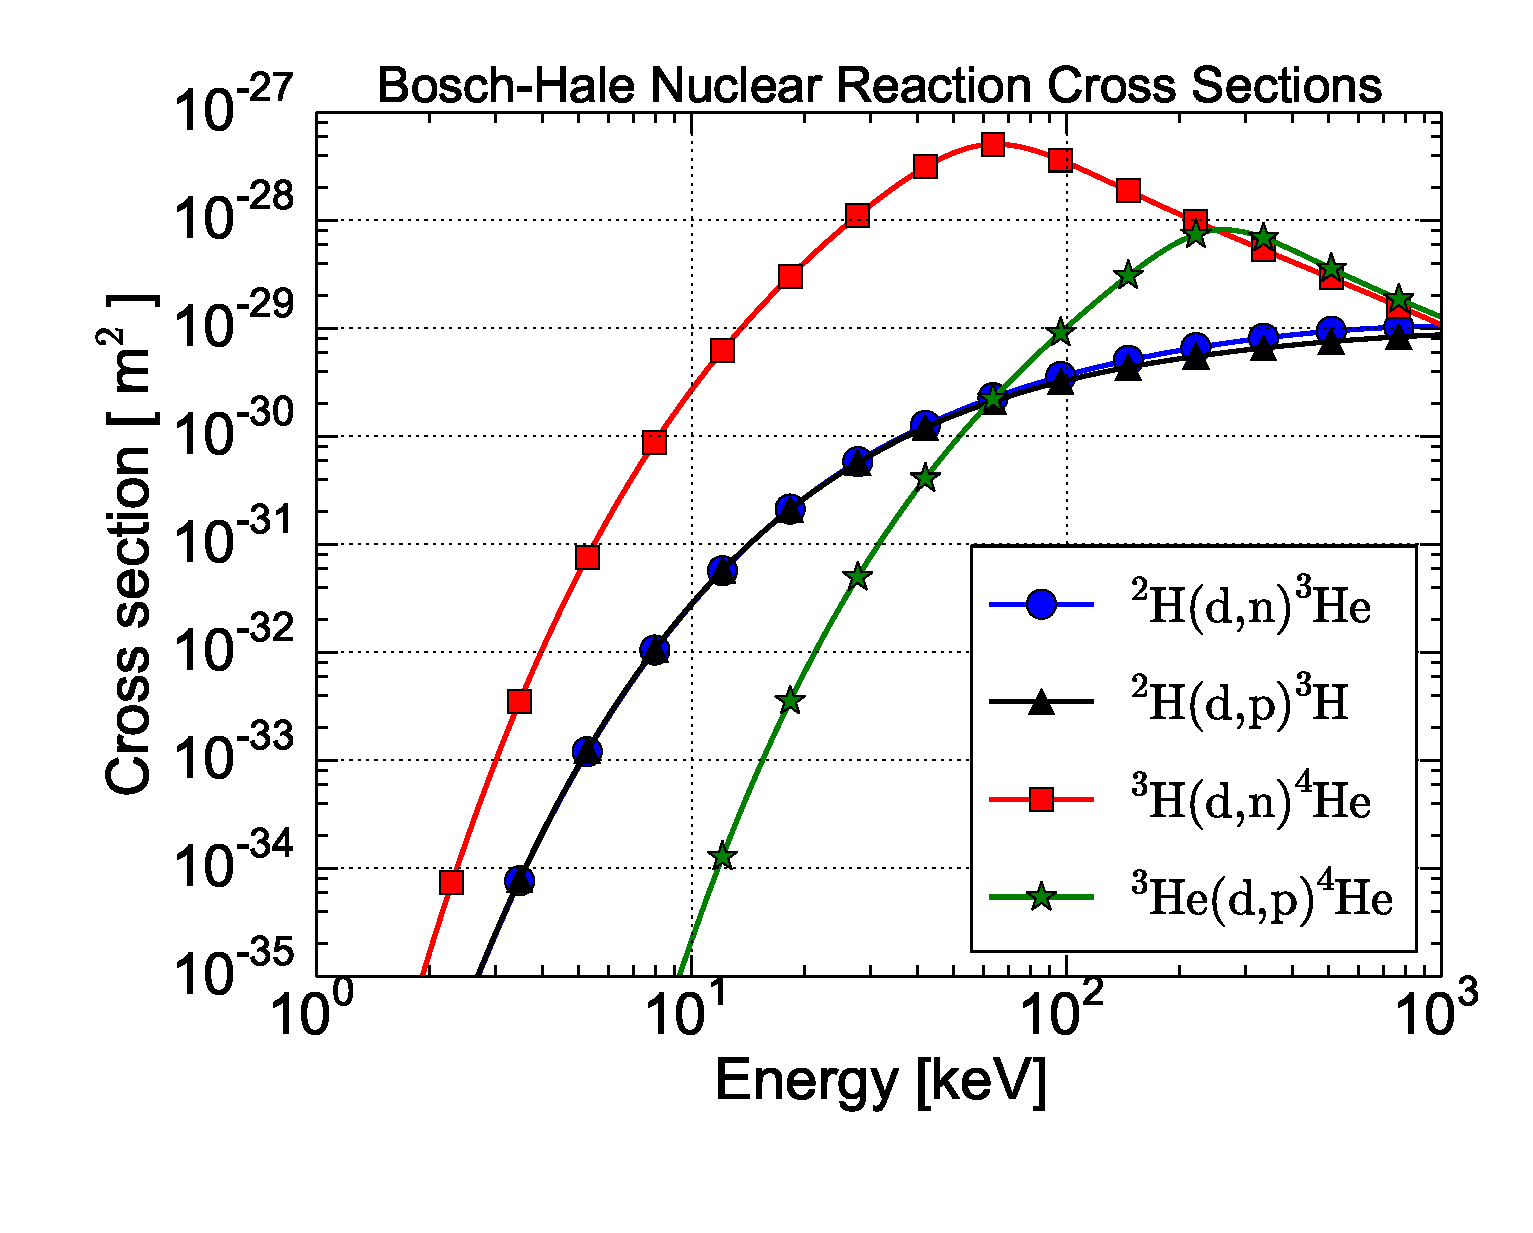
\includegraphics[width=0.95\columnwidth]{figures/BH_CrossSections.eps}
\end{figure}

\index{Reaction rates! Plotted data}
\noindent
\begin{figure}[hb!]
  \centering
  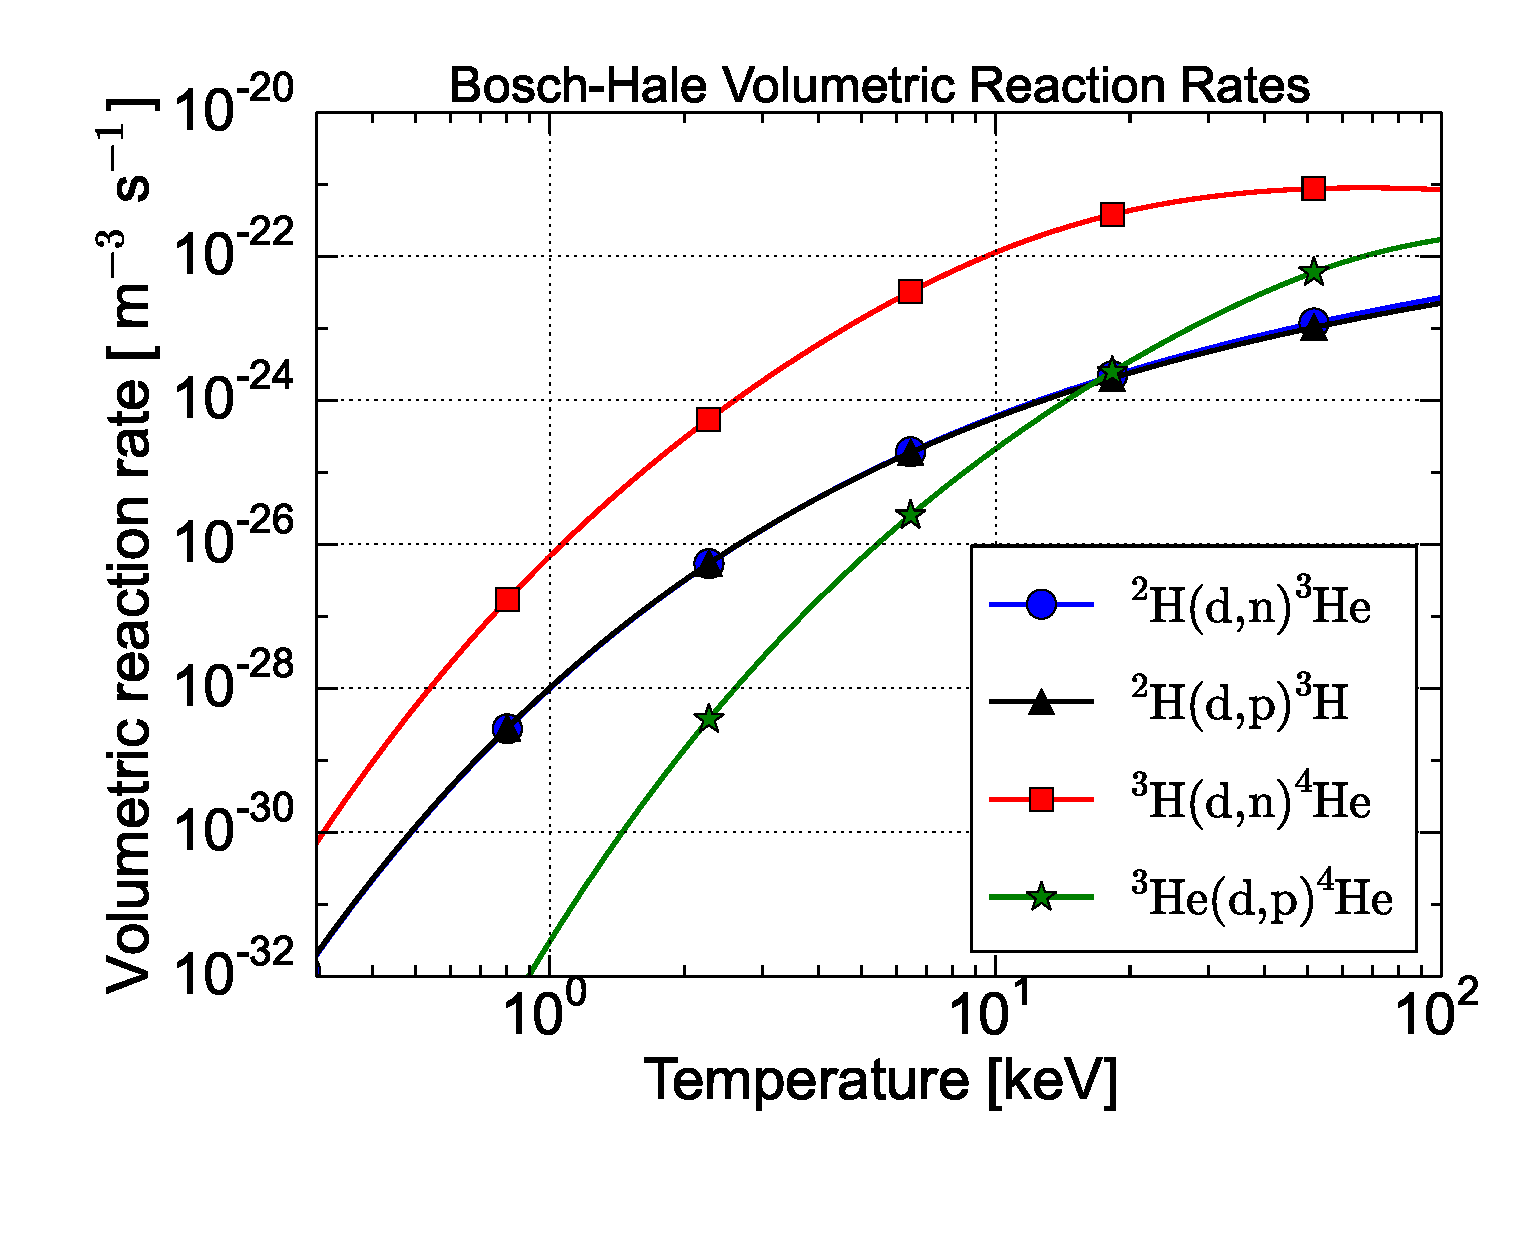
\includegraphics[width=0.95\columnwidth]{figures/BH_ReactionRates.eps}
\end{figure}

\vfill
